\begin{abstract}
Prompt caching bills input tokens a provider has already seen at about a tenth of the list price, and only when a request starts with exactly the bytes of an earlier one. The layout this rewards is now the production default for agents: system prompt and tools first and frozen, every observation appended at the end, nothing reordered, nothing deleted. Because nothing is deleted, a value that changes leaves its old value in the context beside the new one. We ask whether that layout costs accuracy on its own, with the information content held fixed, and whether the cache discount pays for the cost. StaleTrap is a frozen testbed of 144 scripted tool-using episodes (720 question steps, 2,376 tool calls) in which every question is annotated as a stale-trap step, with the update either the agent's own write or an external change revealed only inside a listing row, or a neutral step. Each episode is replayed under four layouts that carry the same information: append-only, relevance-reordered, superseded values redacted in place, and append-only plus a pointer-only session note. Every call is billed and cache-metered by the provider; five directional predictions were logged before the first scored call. First, on Gemini 3.1 Flash-Lite, own-update traps and neutral steps are answered perfectly under every layout, while on external-update traps the append-only layout answers 65.5 percent correctly against 96.0 for redaction, 70.5 for reordering and 73.5 for the note; 34 of 40 audited errors are a superseded value read back, and the gap is as large at six tool calls as at thirty. Second, the append-only layout is the cheapest per episode (1.05 cents against 1.16 for redaction) but redaction is the cheapest per correct episode (1.22 against 1.52) at the billed price and at every counterfactual cache-read price from free to full, because the provider's best-effort cache serves the history on a minority of turns under any layout. Third, across three Gemini generations the append-only layout's external-trap accuracy rises from 40 to 66 to 80 percent and its gap to redaction shrinks from 27 to 18 to 11 points without closing, while redaction stays the cheapest layout per correct episode on every model. The testbed, every episode log, the analysis script and the audit are released.
\end{abstract}

\section{Introduction}
\label{sec:intro}

Production agent stacks are now built around the key-value cache. Providers bill input tokens they have already processed at about a tenth of the list price, and the discount applies only when a request starts with exactly the bytes of an earlier request \citep{a2312_07104,a2601_06007}. The practitioner guidance that followed is specific: put the system prompt and the tool declarations first and never change them, append every new observation at the end, mask tools instead of removing them, and never reorder or delete earlier blocks \citep{manus2025,anthropic2025context}. This paper calls that layout the cache-optimal layout.

The layout has a side effect that the guidance does not price. Nothing is ever removed, so when a value changes, the old value stays in the context next to the new one. A model that must answer from its context then has to prefer the later of two values for the same field. We know this is hard in general: the latest of several revisions of one fact is retrieved less reliably as revisions accumulate \citep{a2603_12271,a2510_22752}, and agents answer from observations the world has overtaken \citep{a2610_05281}. We do not know whether the cache discipline itself, with the information content held fixed, costs accuracy, or what that cost is worth against the cache it protects. The context-management literature prunes or masks old observations and reports accuracy, but prices tokens at list rates with no cache term \citep{a2606_10209,a2508_21433,a2605_18854}; the caching literature reports cost and latency and no accuracy \citep{a2601_06007,a2607_15516}.

We answer the question with a controlled replay. StaleTrap is a deterministic tool environment with 144 scripted episodes in which, for every question the agent answers, we know by construction whether a superseded value for the queried field is in its context and whether the update was the agent's own write or an external change revealed only inside a listing row. Each episode is replayed under four layouts that carry the same information: the cache-optimal append-only layout (L1), a relevance-reordered layout (L2), a layout that redacts superseded values in place (L3), and the append-only layout plus a pointer-only session note (L4). Every call is billed and cache-metered by the provider, and five directional predictions were logged before the first scored call.

The answer has two halves. On the model with the full grid, Gemini 3.1 Flash-Lite, own-update traps and neutral steps are answered perfectly under every layout, so the cache discipline is free whenever the agent's own tool replies carry the current value. On external-update traps the append-only layout answers 65.5 percent correctly, the redacting layout 96.0, the reordered layout 70.5 and the note 73.5, and 34 of 40 audited wrong answers are a superseded value read back. The cost half reverses the expected trade: the append-only layout is the cheapest per episode, but the redacting layout is the cheapest per correct episode at the billed price and at every counterfactual cache-read price, because on Google's best-effort cache the history is rarely served from cache under any layout. Across three Gemini generations the gap shrinks from 27 to 11 points but does not close, and redaction stays cheapest per correct episode on every model.

Our contributions are:
\begin{enumerate}
\item \textbf{StaleTrap}, a frozen, hash-manifested testbed of 144 scripted tool-using episodes (720 questions, 2,376 tool calls) in which every question step is annotated as a stale-trap step (own or external update) or a neutral step (Section~\ref{sec:method}).
\item A \textbf{content-fixed layout factorial} (order only, content only, recitation only) scored against provider-billed cost and cached tokens, with a within-task paired analysis and one pre-registered test family (Section~\ref{sec:method}, Appendix~\ref{app:tests}).
\item The finding that \textbf{the accuracy cost of the cache-optimal layout is confined to external updates}: zero on own updates and neutral steps, 30.5 points on external updates for Gemini 3.1 Flash-Lite, with 34 of 40 audited errors being a superseded value read back (Section~\ref{sec:results}).
\item The finding that \textbf{redaction is cheaper per correct episode at every cache-read price} on the tested models, which reverses the pre-registered price-threshold prediction and is explained by the measured per-turn cache behaviour (Section~\ref{sec:results}).
\item A scored pre-registration (Section~\ref{sec:prereg}) and a narrated account of what the design cannot show (Section~\ref{sec:limits}).
\end{enumerate}

\begin{figure}[t]
\centering
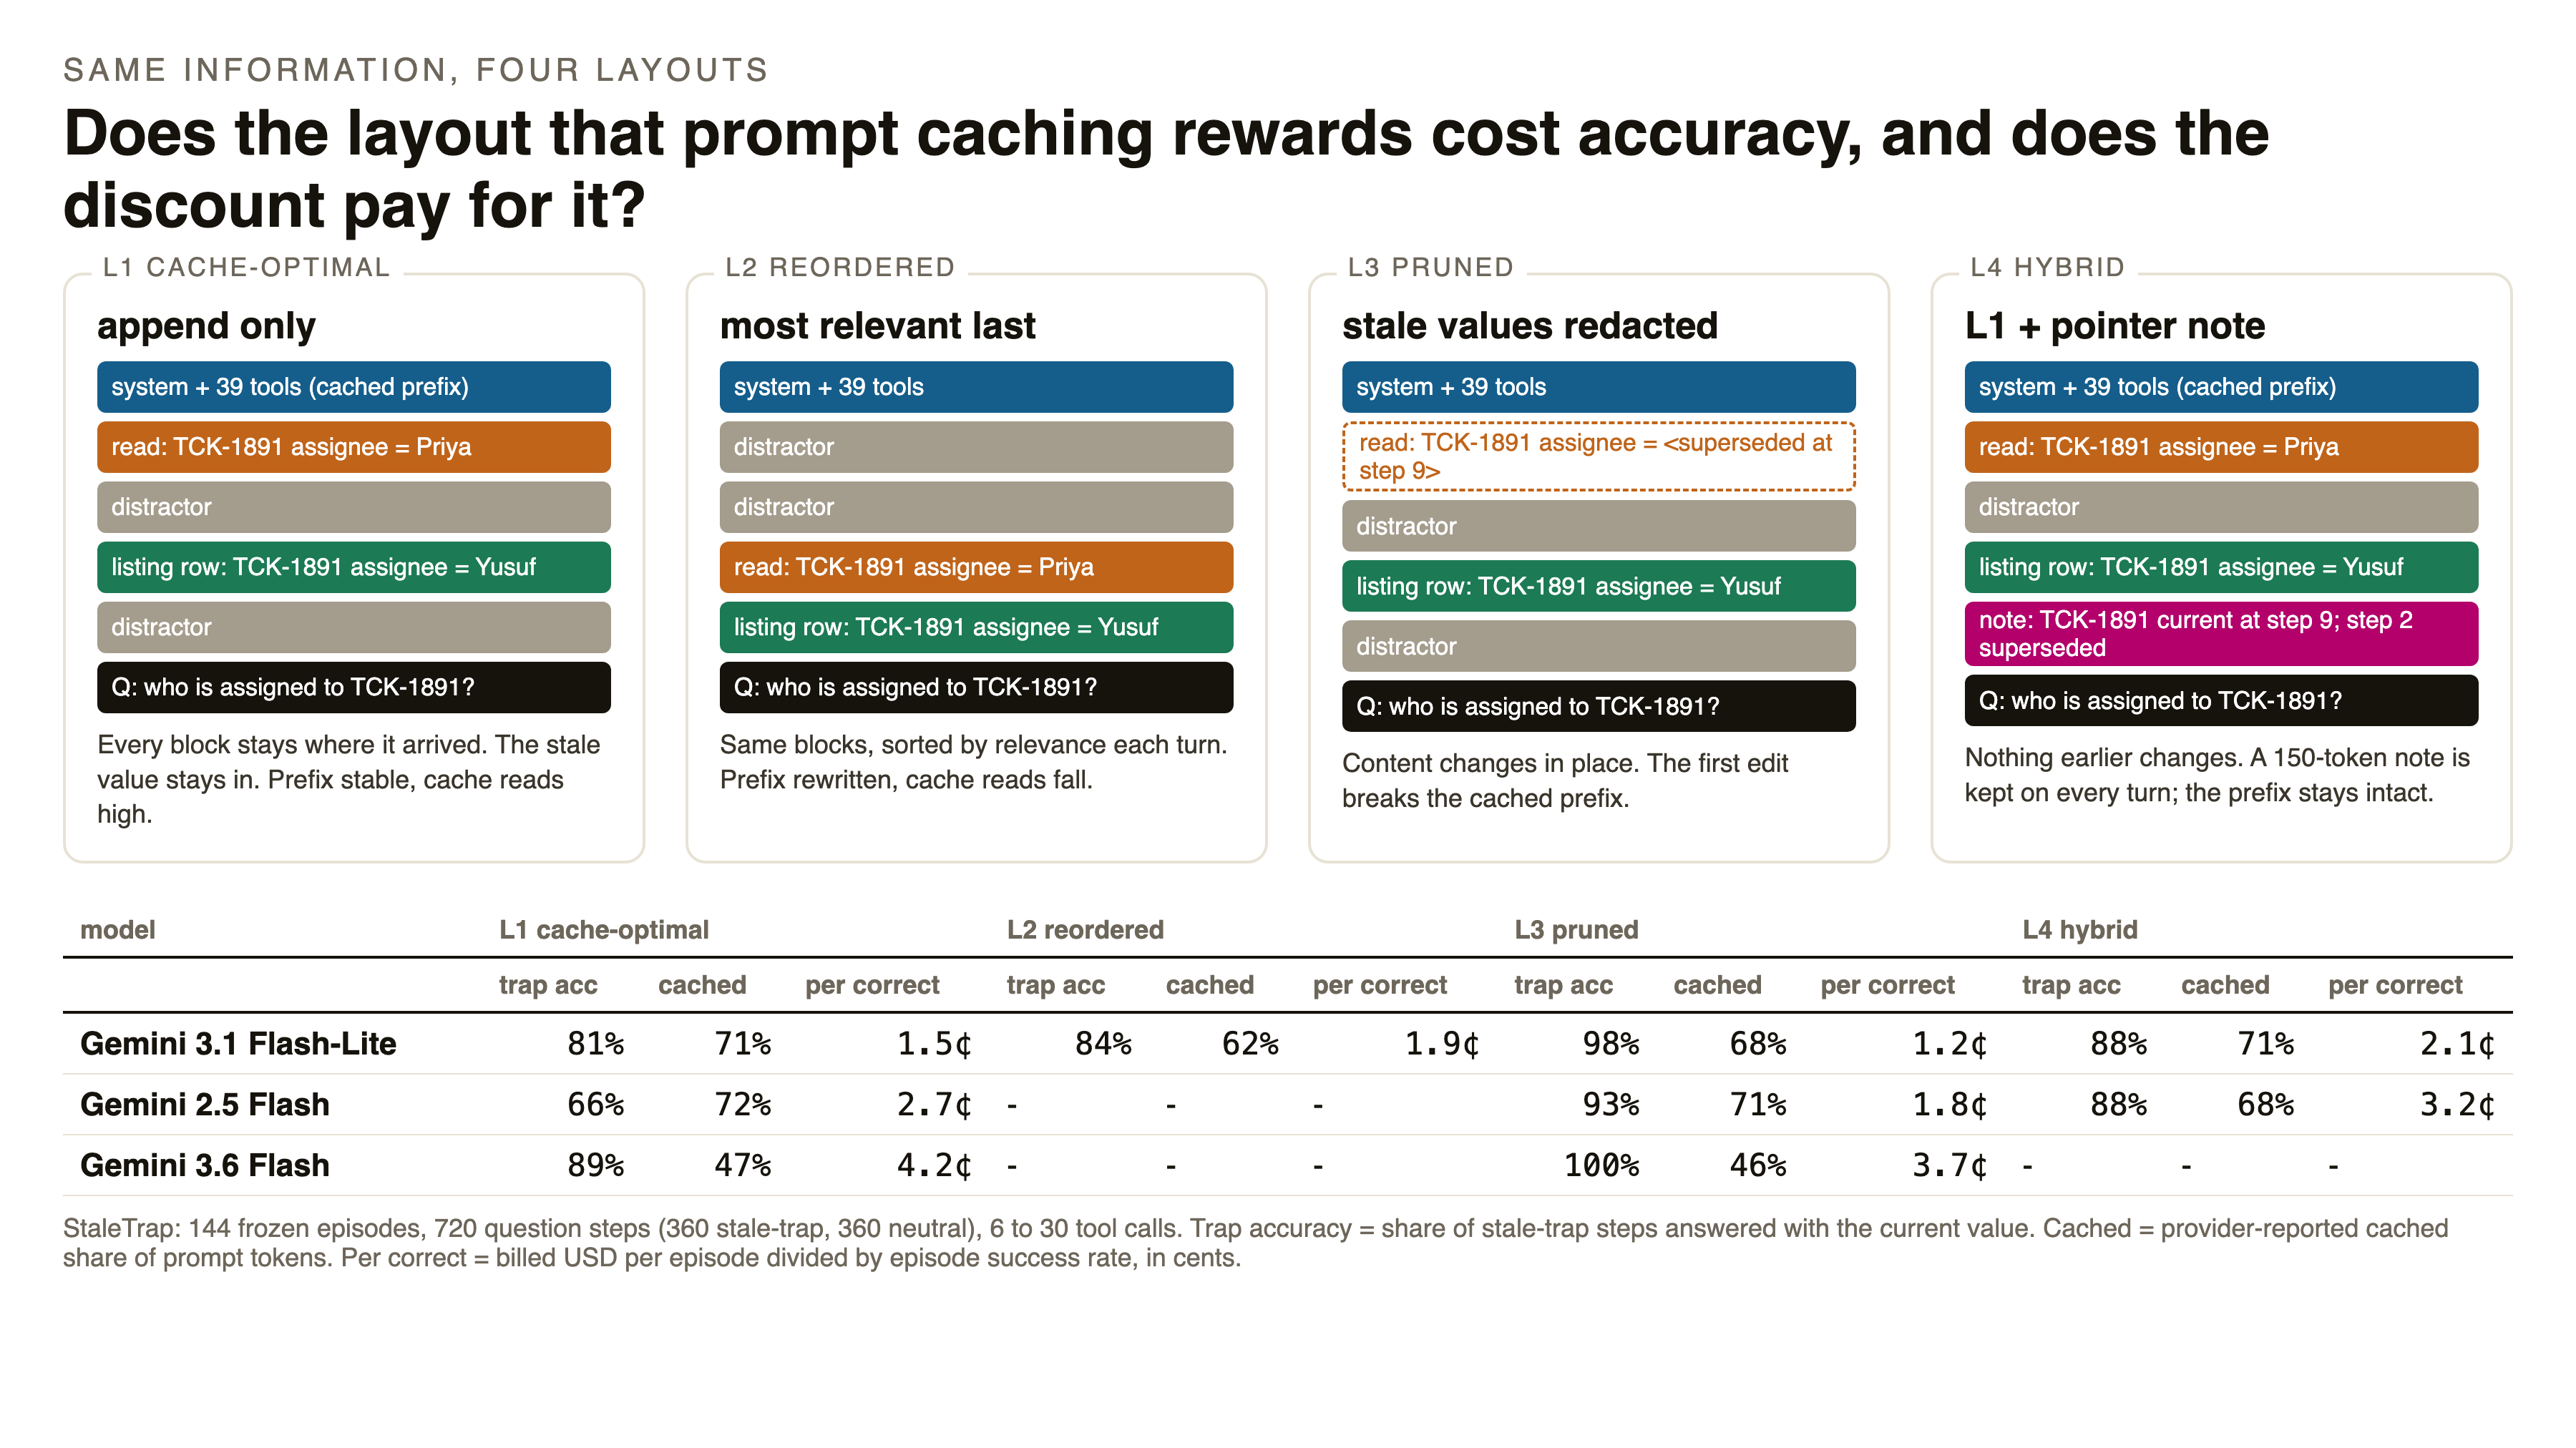
\includegraphics[width=0.92\textwidth]{assets/fig1_teaser.png}
\caption{Study design and headline numbers. One scripted agent episode is replayed under four context layouts that carry the same information. L1 keeps every observation in arrival order (the layout that prompt caching rewards). L2 reorders earlier blocks by relevance. L3 redacts values that a later result has replaced. L4 keeps L1 and appends a short note saying which earlier observations are current. Each question step is scored against the live state of the environment, and every call is billed and cache-metered by the provider.}
\label{fig:teaser}
\end{figure}

\section{What was known and what is new}
\label{sec:known}

Three things are established, and we do not claim them. Models use the start and the end of a long context better than its middle \citep{a2307_03172,a2406_16008}, and the latest value of a fact revised several times inside one context is retrieved less reliably as revisions accumulate \citep{a2603_12271,a2510_22752}. Agents answer from tool observations that the world has since overtaken \citep{a2610_05281}, and removing or masking old observations changes accuracy in a model-dependent way \citep{a2606_00408,a2606_10209,a2508_21433}. Prompt caching cuts the cost of long agent sessions by 40 to 80 percent, and the discount is lost when earlier bytes change \citep{a2601_06007,a2607_15516,a2608_00101}.

What was not known is whether the layout discipline that caching imposes costs accuracy on its own, with the information content held fixed. Table~\ref{tab:delineation} (Appendix~\ref{app:delineation}) lists the nearest work. The closest paper measures provider-billed cost split into cache creation and reads against task success and shows that compressing tool outputs can raise the bill by changing trajectories \citep{a2607_12161}; it varies compression, which changes content, not layout. The one evaluation of caching strategies for long agent tasks reports cost and latency and no accuracy \citep{a2601_06007}. The context-management papers that report accuracy price tokens at list rates with no cache term, so every published ``compression saves X percent'' is biased against append-only layouts by the cache-read discount \citep{a2606_10209,a2605_18854,a2504_13359,a2510_11977}. Relevance reordering was no better than shuffling in realistic retrieval \citep{a2505_15561}, but without a history or a cache. \textbf{Ours alone:} a content-fixed manipulation of layout (order only, content only, recitation only) in a multi-turn tool-using agent, scored against provider-reported cached tokens and billed dollars, with every question step annotated as a stale-trap step or a neutral step, and a per-model answer to whether a cache-read price exists at which the cheapest layout per call stops being the cheapest per correct answer. \textbf{Who is affected:} anyone who followed the 2025 guidance to design around the KV cache \citep{manus2025,anthropic2025context}. If the append-only layout loses accuracy only where the world changed behind the agent, the cost of caching discipline becomes a known quantity with a known fix; if it loses none, the pruning literature's cost numbers need a cache term.

\section{Method}
\label{sec:method}

\paragraph{The question in one sentence.} Hold the information in an agent's context fixed, change only how it is laid out, and measure what happens to accuracy, cache reads and the bill.

\paragraph{Why a self-built testbed.} To attribute an error to a stale value, we must know, for every question the agent answers, whether a superseded value for the queried field is sitting in its context. Public agent benchmarks do not annotate this. We therefore built StaleTrap, a deterministic tool environment with scripted episodes in which that annotation is known by construction and the testbed was frozen, with a recorded hash, before any scored episode ran.

\paragraph{Environment.} Three back-office domains (warehouse inventory, a shared meeting calendar, a support-ticket queue) are exposed as 29 JSON-schema tools: 10 reads, 19 writes. A fourth domain of 10 messaging and HR tools is present in every call and never required by any task, so the catalogue is masked by the agent's choice rather than trimmed per step, as production stacks do. A local executor holds the state and returns realistic JSON. Every result declares which (record, field) values it states: a dedicated read states the fields it returns, a write states the field it changed and reports the new value, and a listing states the fields of every row it contains. The shared prefix (system prompt plus tool declarations) measures 5,102 tokens on Google's tokenizer, above every provider's minimum for implicit caching. Appendix~\ref{app:prompts} prints it verbatim.

\paragraph{Episodes.} An episode is a scripted session of user instructions. Most instructions ask for one tool call ("Record that we received 22 units of SKU-2249"). Some are no-tool questions ("Based only on the information already gathered in this conversation, and without calling any tools, what is the current on-hand quantity of SKU-2249?"), served with tool calling disabled, answered as a one-key JSON object and scored by exact match against the executor's live state after canonicalisation. A \textbf{trap thread} reads a record's field, later updates it one to three times, and then asks for its current value, so that a superseded value is present in context when the question arrives. A \textbf{neutral thread} reads a field once and asks for it later, so that nothing in context competes. Trap threads come in two kinds. In an \emph{own} update, the agent's own write returns the new value explicitly. In an \emph{external} update, someone else changes the record and the agent only ever sees the new value as one row inside an unrelated listing it was asked to fetch (a bin inventory, a room schedule, a ticket queue). The second kind is the realistic source of stale observations \citep{a2610_05281}; five of nine task templates use it and four use own updates. The remaining calls are distractors. At the \emph{low} level they are compact reads and writes on unrelated records. At the \emph{high} level they are verbose listings, reads of near-miss identifiers that differ by one transposed digit, and writes to other fields of the very records the questions are about. Episode length is 6, 12, 18 or 30 tool calls, with 2, 4, 6 or 8 questions, and the distance from the last update to its question grows with length (2 to 3, 3 to 6, 3 to 7, 4 to 9 calls). The grid is 3 domains by 3 templates by 4 lengths by 2 distractor levels by 2 seeds: 144 episodes, 720 questions (360 trap, 360 neutral), 2,376 tool calls. Every task has two phrasings. A script verifies that every stale value in every trap differs from the final answer (360 of 360).

\paragraph{Layouts.} Each turn, the runner rebuilds the message list from the transcript so far under one of four rules; the agent's own replies and tool results are never altered except as the rule states, and the information content is identical for L1, L2 and L4. \textbf{L1} is the cache-optimal layout: system prompt and tools first, every block in arrival order, newest observation and user turn last, tools masked by \texttt{tool\_choice} rather than removed. \textbf{L2} keeps the same blocks but stable-sorts the earlier ones by how many record identifiers they share with the current turn, most relevant last; the prefix is rewritten every turn. \textbf{L3} keeps arrival order and redacts, in place, every value that a later result has restated (``\textless superseded at step 7\textgreater''); a result whose stated values are all superseded becomes one placeholder line. The rule is schema-level and transcript-derived, which makes it an upper bound for any real pruner, and it edits earlier bytes, so the cached prefix breaks at the first edit. \textbf{L4} is L1 plus a pointer-only session note prepended to every user turn and kept there, so the history stays append-only: the session goal, the step number, and for every record with more than one observation which step is current and which steps are superseded. The note never contains a value, so it cannot leak an answer. It adds about 150 tokens per turn, and because earlier notes are never rewritten the prefix stays intact; the price is that every earlier note stays in the history, so an L4 episode sends more prompt tokens than an L1 episode (Section~\ref{sec:results} reports how many). Appendix~\ref{app:layouts} shows one episode serialised under each layout.

\paragraph{Models and protocol.} The plan froze three model families (Google, Anthropic, OpenAI). The OpenRouter workspace used for this study carries a guardrail that returns ``no endpoints match your guardrail restrictions'' for every non-Google model; it was probed before the plan was frozen and again after the main grid, and the plan's stated fallback applies: a one-family capability ladder. Gemini 3.1 Flash-Lite runs the full grid (144 tasks by 4 layouts, 576 episodes). Gemini 2.5 Flash, an older generation with thinking enabled, runs L1, L3 and L4 on the seed-0 half of the grid (72 tasks, 216 episodes). Gemini 3.6 Flash, the newest generation, runs L1 and L3 on a 36-task subset balanced over domain, template, length and distractor (72 episodes). Gemini 3.5 Flash-Lite was smoke-tested and dropped because it returns malformed function calls on about a third of tool-calling turns with our 39-tool catalogue. The Anthropic cache on/off control could not run; Section~\ref{sec:results} reports the Google substitute. All calls go through OpenRouter with temperature 0, reasoning effort minimal, 700 output tokens of headroom, a per-episode session identifier for sticky routing, and turns strictly sequential inside one process so that the cache never expires between turns. On Anthropic we place explicit cache breakpoints on the system block and on the newest user turn; on OpenAI caching is automatic; on Google it is implicit, because an explicit breakpoint on Gemini creates a billed cache on every call (we measured 3.5 to 5.8 times the cost of an implicit hit). Every call logs the provider's prompt, cached, cache-write, completion and reasoning token counts and the billed dollar amount (\texttt{usage.cost}); no cost in this paper is modelled from a price sheet except where the text says counterfactual.

\paragraph{Analysis.} The unit is the task. For each model we form within-task paired differences between layouts on five quantities: accuracy on stale-trap steps, accuracy on neutral steps, episode success (all questions right), billed dollars, and the cached share of prompt tokens. We report two-sided sign-flip permutation tests over tasks (20,000 flips), task-bootstrap 95 percent intervals (10,000 resamples), paired $d_z$, and, as a robustness column, an exact sign-flip over the nine task templates. Interactions are tested directly by label permutation: the trap gap by length (slope per call), by distractor level, trap against neutral (a difference of differences), and by model family. Benjamini-Hochberg runs over the full family of primary tests from the first run, and only survivors are bolded. For the cost side we compute dollars per correct task from billed cost, then recompute it under counterfactual cache-read prices from 0 to 1 times the input price to find where the cheapest layout changes. Forty wrong answers are hand-coded from their observation history as stale value, reveal not executed, ambiguous, arithmetic, wrong record or abstention, and shipped with the release. Two sensitivity checks guard the main contrast: trap accuracy restricted to questions whose scripted thread steps the agent actually executed (an agent that skips a listing call never sees the fresh value), and, in place of the cache on/off control, trap accuracy on question turns that Google's best-effort cache served from cache against those it did not, paired within question on the repeat battery.

\paragraph{Pre-registration.} Five directional predictions were written into the project log before any model call (Appendix~\ref{app:prereg}). We report each as confirmed, reversed or not supported in Section~\ref{sec:prereg}.

\section{Results}
\label{sec:results}

Table~\ref{tab:main} gives the per-layout means for every model and Table~\ref{tab:contrasts} the paired contrasts for the model that ran the full grid. Bold entries survive Benjamini-Hochberg over the family of The family holds 65 tests; 29 survive Benjamini-Hochberg at $q = 0.05$ (effective threshold $p \le 0.0207$).


\begin{table}[t]
\centering\small
\begin{tabular}{llrrrrrrr}
\toprule
\textbf{Model} & \textbf{Layout} & $n$ & \textbf{Trap acc.} & \textbf{Neutral acc.} & \textbf{Success} & \textbf{Cents/episode} & \textbf{Cents/correct task} & \textbf{Cached share} \\
\midrule
Gemini 2.5 Flash & L1 append-only & 72 & 0.660 & 1.000 & 0.528 & 1.43 & 2.71 & 0.716 \\
 & L3 pruned & 72 & 0.933 & 1.000 & 0.861 & 1.54 & 1.78 & 0.710 \\
 & L4 hybrid & 72 & 0.875 & 1.000 & 0.778 & 2.45 & 3.15 & 0.683 \\
\midrule
Gemini 3.1 Flash-Lite & L1 append-only & 144 & 0.806 & 1.000 & 0.694 & 1.05 & 1.52 & 0.708 \\
 & L2 reordered & 144 & 0.841 & 1.000 & 0.729 & 1.35 & 1.85 & 0.619 \\
 & L3 pruned & 144 & 0.983 & 1.000 & 0.944 & 1.16 & 1.22 & 0.676 \\
 & L4 hybrid & 144 & 0.879 & 1.000 & 0.771 & 1.60 & 2.07 & 0.711 \\
\midrule
Gemini 3.6 Flash & L1 append-only & 36 & 0.889 & 1.000 & 0.833 & 3.51 & 4.21 & 0.475 \\
 & L3 pruned & 36 & 1.000 & 0.972 & 0.972 & 3.57 & 3.67 & 0.464 \\
\bottomrule
\end{tabular}

\caption{Per-layout means. Trap and neutral accuracy are per-question means over episodes; success is the share of episodes with every question right; cost is the provider-billed amount per episode; cached share is cached prompt tokens over prompt tokens, summed over the episode. Gemini 2.5 Flash ran 72 tasks under L1, L3 and L4; Gemini 3.6 Flash ran 36 tasks under L1 and L3.}
\label{tab:main}
\end{table}

\begin{table}[t]
\centering\scriptsize
\resizebox{\textwidth}{!}{\begin{tabular}{lrrrrr}
\toprule
\textbf{Contrast} & \textbf{Trap acc.} & \textbf{Neutral acc.} & \textbf{Success} & \textbf{USD/episode} & \textbf{Cached share} \\
\midrule
L1 $-$ L2 (order) & -0.036 [-0.079, 0.006], $p$=0.116 & +0.000 [0.000, 0.000], $p$=1.000 & -0.035 [-0.090, 0.021], $p$=0.334 & \textbf{-0.30c [-0.36, -0.24], $p$=$<$0.0001} & \textbf{+0.089 [0.074, 0.103], $p$=$<$0.0001} \\
L1 $-$ L3 (content) & \textbf{-0.177 [-0.230, -0.128], $p$=$<$0.0001} & +0.000 [0.000, 0.000], $p$=1.000 & \textbf{-0.250 [-0.326, -0.180], $p$=$<$0.0001} & \textbf{-0.10c [-0.15, -0.06], $p$=$<$0.0001} & \textbf{+0.032 [0.018, 0.045], $p$=$<$0.0001} \\
L4 $-$ L1 (note) & \textbf{+0.073 [0.031, 0.120], $p$=0.0013} & +0.000 [0.000, 0.000], $p$=1.000 & +0.076 [0.014, 0.139], $p$=0.034 & \textbf{+0.54c [0.44, 0.65], $p$=$<$0.0001} & +0.003 [-0.010, 0.015], $p$=0.642 \\
L4 $-$ L3 & \textbf{-0.104 [-0.145, -0.066], $p$=$<$0.0001} & +0.000 [0.000, 0.000], $p$=1.000 & \textbf{-0.174 [-0.243, -0.111], $p$=$<$0.0001} & \textbf{+0.44c [0.35, 0.53], $p$=$<$0.0001} & \textbf{+0.035 [0.019, 0.050], $p$=$<$0.0001} \\
L2 $-$ L3 & \textbf{-0.141 [-0.188, -0.098], $p$=$<$0.0001} & +0.000 [0.000, 0.000], $p$=1.000 & \textbf{-0.215 [-0.285, -0.146], $p$=$<$0.0001} & \textbf{+0.19c [0.15, 0.24], $p$=$<$0.0001} & \textbf{-0.057 [-0.069, -0.044], $p$=$<$0.0001} \\
\bottomrule
\end{tabular}
}
\caption{Paired within-task contrasts on Gemini 3.1 Flash-Lite (144 tasks): mean difference, task-bootstrap 95 percent interval, two-sided sign-flip $p$. Bold survives BH. Cost differences are in cents.}
\label{tab:contrasts}
\end{table}

\paragraph{The cost of the cache-optimal layout is confined to external updates.} On Gemini 3.1 Flash-Lite, L1 answers 80.6 percent of trap questions [75.0, 85.8] and L3 answers 98.3 percent [96.9, 99.4]; the paired difference is $-0.177$ [$-0.231$, $-0.127$], sign-flip $p < 10^{-4}$, $d_z = -0.55$ (Table~\ref{tab:contrasts}). Neutral questions are answered perfectly under every layout, so the trap-minus-neutral difference of differences equals the trap gap and is as significant. Splitting the trap questions by kind (Figure~\ref{fig:stale}, Table~\ref{tab:cells_chain}) locates the entire effect: the 160 own-update traps are answered perfectly under every layout, and on the 200 external-update traps L1 scores 65.5 percent, L2 70.5, L3 96.0 and L4 73.5. When the agent's own tool reply states the current value, the stale copy beside it does no harm. When the current value arrived as one row of a listing the agent fetched for another reason, the append-only agent answers from its own earlier write about one time in three. The gap does not grow with episode length (slope $+0.0006$ per call, label-permutation $p = 0.85$; the gap is $-0.22$ at six calls and $-0.22$ at thirty, Table~\ref{tab:cells_length}, Figure~\ref{fig:dose}) and does not depend on the distractor level (high minus low $-0.035$, $p = 0.54$). The stale value costs what it costs as soon as it exists.

\begin{figure}[t]
\centering
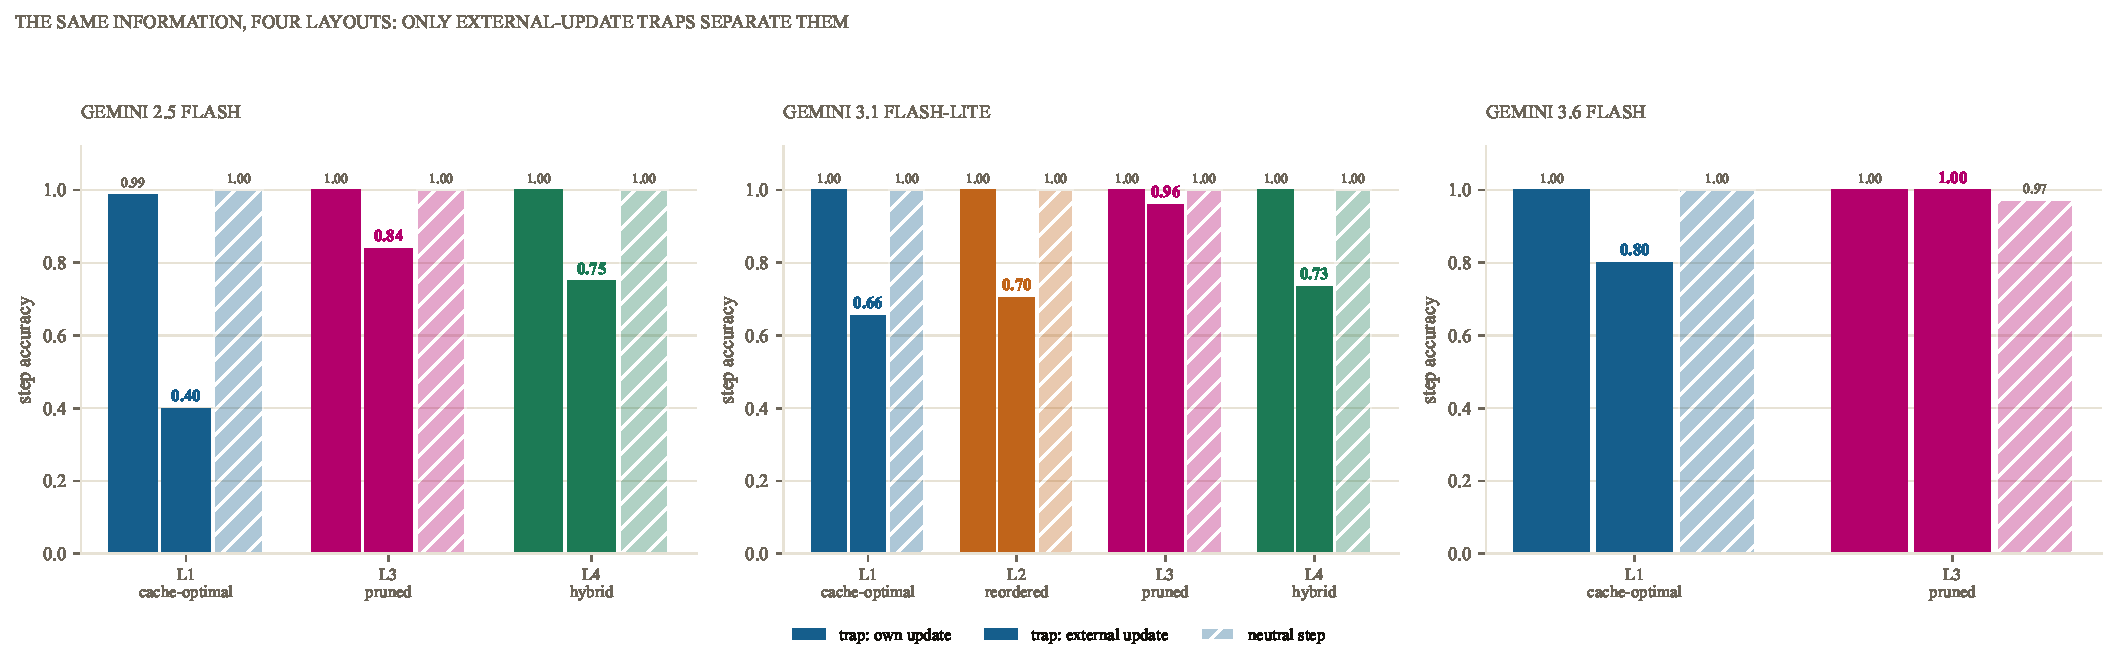
\includegraphics[width=\textwidth]{assets/fig2_stale.pdf}
\caption{Step accuracy by layout on own-update traps, external-update traps and neutral steps, per model. Only the external-update bars move.}
\label{fig:stale}
\end{figure}

\paragraph{Order alone does nothing; the note recovers a quarter.} Reordering earlier blocks by relevance (L2) does not improve on L1: $-0.036$ [$-0.080$, $+0.006$], $p = 0.11$, and it rewrites the prefix every turn. The pointer-only note (L4) improves on L1 by $+0.073$ [$+0.031$, $+0.120$], $p = 0.001$, which is 42 percent of the L1-to-L3 gap over all traps [21, 60] and 26 percent on external traps, while keeping L1's cached share exactly (ratio 1.00). L4 remains far from L3 ($-0.104$, $p < 10^{-4}$). The note is also the layout whose gap to L1 shrinks with length (slope $-0.0065$ per call, $p = 0.012$): it helps most in short episodes and least at thirty calls, where the accumulated notes are longest.

\paragraph{What the wrong answers are.} The hand audit (Appendix~\ref{app:audit}) coded 40 wrong trap answers, including every wrong L3 answer: 34 are a superseded value read back, almost always the agent's own earlier write with the overtaking listing row ignored; 3 are threshold questions where the fresh quantity equals the threshold, so a stale read and a strict-inequality misreading coincide; 2, both under L3, are questions whose scripted listing call the agent had skipped, so the fresh value never entered its context; 1 is a derived number. Reveal steps were executed 99.0 to 100 percent of the time under every layout, and restricting to fully executed threads moves no layout's trap accuracy by more than half a point (Table~\ref{tab:fidelity}). The repeat battery finds a cell's trap outcome flipping between identical temperature-0 runs in 11 percent of cells (within-cell standard deviation of question accuracy 0.017); the phrasing battery finds $-0.007$ [$-0.042$, $+0.032$] between the two phrasings (Appendix~\ref{app:batteries}).

\paragraph{The bill reverses between per episode and per correct episode.} L1 is the cheapest layout per episode at 1.05 cents [0.97, 1.14]; L3 costs 1.16 cents [1.06, 1.26], a paired difference of $+0.10$ cents [0.06, 0.15], $p < 10^{-4}$; L2 costs 1.35 and L4 1.60. Per correct episode the order is L3 1.22 cents, L1 1.52, L2 1.85, L4 2.07 (Table~\ref{tab:main}, Figure~\ref{fig:frontier}). L1 and L3 are the two points on the Pareto frontier; L2 and L4 are dominated. Repricing every cached token at multiples of the input price from 0 to 1 (Table~\ref{tab:d5}, Figure~\ref{fig:threshold} in Appendix~\ref{app:figs}) never changes the ranking: L3 is the cheapest per correct episode at every multiplier. There is no cache-read price on this provider at which the cache-optimal layout pays for its errors. The modelled cost at list prices reproduces the billed cost to the fourth decimal, which confirms that the provider bills exactly what it reports.

\begin{figure}[t]
\centering
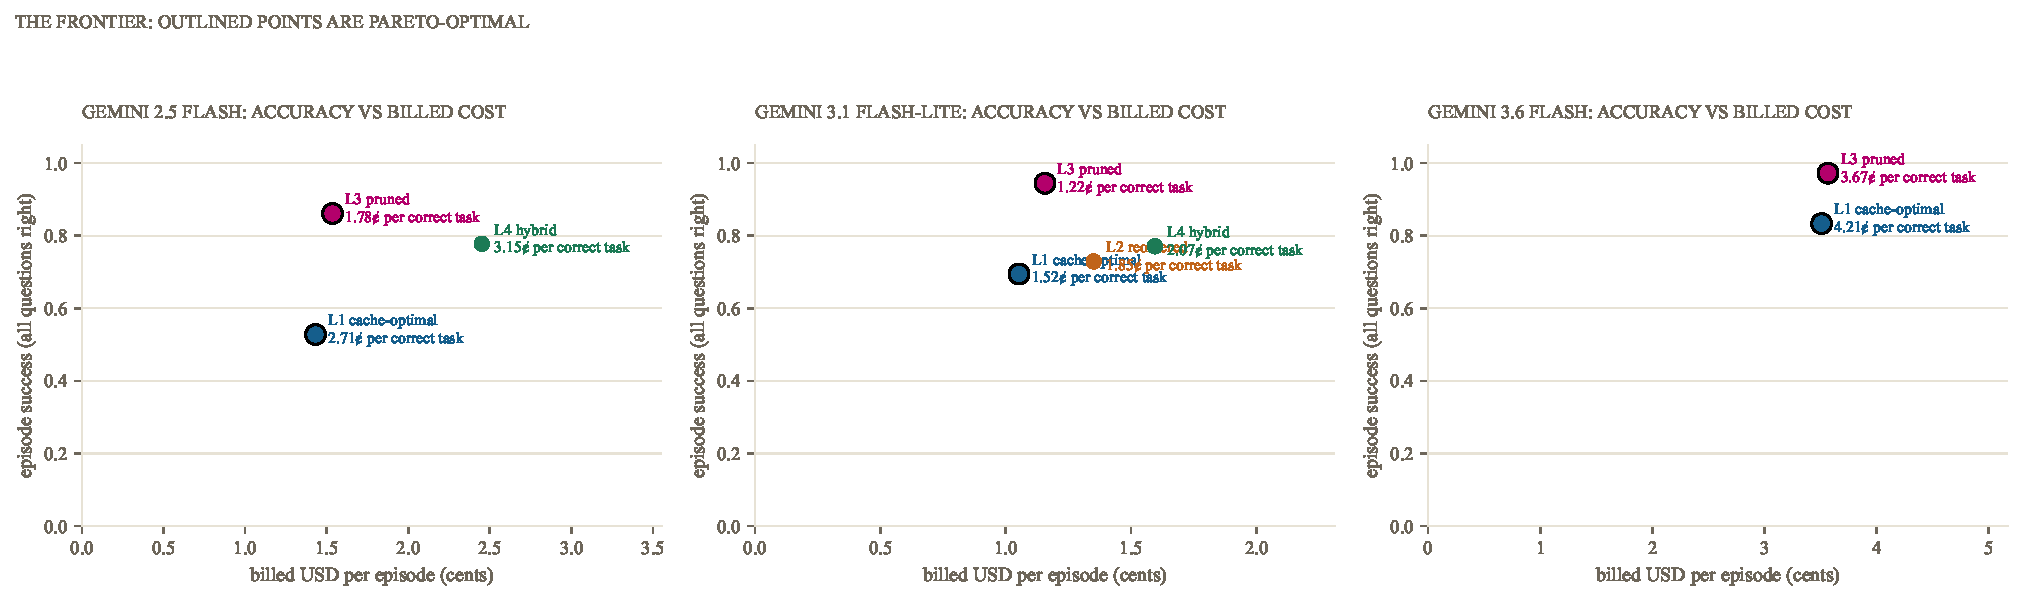
\includegraphics[width=\textwidth]{assets/fig3_frontier.pdf}
\caption{Episode success against billed cents per episode, per model; outlined points are Pareto-optimal; cents per correct episode annotated.}
\label{fig:frontier}
\end{figure}

\paragraph{Why: the history is rarely cached under any layout.} Figure~\ref{fig:cache} (Appendix~\ref{app:figs}) shows the cached share of prompt tokens by turn. Over an episode the share is 0.71 under L1 and 0.68 under L3 (paired $+0.032$ [0.019, 0.046]); under L2 it is 0.62 and under L4 0.71. Most of that share is the 5,100-token static prefix. Counting only the history, the cached share is 0.24 under L1, 0.13 under L2, 0.15 under L3 and 0.45 under L4 (Table~\ref{tab:main}). Google's implicit cache serves the growing history on a minority of turns even when the bytes are unchanged, so the layout that caching rewards is rewarded for its history by nine percentage points over L3, and L3's shorter prompts (118k against 122k tokens per episode) recover most of that. Two further facts shape the bill. No-tool question turns are served from cache far less often than tool turns (hit rate 0.51 against 0.93 under L1; 0.15 under L2; 0.37 under L3; 0.69 under L4), because disabling tool choice changes the request. And the L4 note, which must stay in the history to keep the prefix stable, raises prompt tokens per episode by 69 percent over L1 and the bill by 51 percent: the quadratic cost of a note repeated on every turn is what puts L4 off the frontier, not a cache loss.

\paragraph{Caching does not change the answers.} The on/off control could not run (Section~\ref{sec:method}). In its place, the best-effort cache itself provides a comparison at identical bytes: the same question, same layout, served from cache in some runs of the repeat battery and not in others. Paired within question, the difference in trap accuracy is 0.000 over the 11 questions that saw both outcomes ($p = 1$). The unpaired comparison over the main grid is confounded, because cache hits concentrate in the later turns of long episodes where traps are harder; it shows $-0.03$ ($p = 0.56$) under L1 and $-0.12$ ($p = 0.001$) under L4 before stratification and $-0.004$ and $-0.063$ after stratifying by length and chain. We read this as no evidence that a cache hit changes an answer, with the caveat that the paired sample is small.

\subsection{Three Gemini generations}
\label{sec:ladder}
Gemini 2.5 Flash (older generation, thinking on, 72 tasks under L1, L3 and L4) and Gemini 3.6 Flash (newest generation, 36 tasks under L1 and L3) bracket the main model (Table~\ref{tab:main}, Figure~\ref{fig:stale}). External-trap accuracy under L1 rises with generation: 0.40 on 2.5 Flash (100 questions), 0.655 on 3.1 Flash-Lite (200) and 0.80 on 3.6 Flash (40); under L3 it is 0.84, 0.96 and 1.00. Own-update traps and neutral steps stay at or near 1.00 everywhere (one own-update miss on 2.5 Flash under L1, one neutral miss on 3.6 Flash under L3). The paired L1 minus L3 trap gap is $-0.273$ [$-0.367$, $-0.186$] on 2.5 Flash, $-0.177$ on 3.1 Flash-Lite and $-0.111$ [$-0.213$, $-0.028$] on 3.6 Flash ($p = 0.031$ on 36 tasks). Permuting model labels over the task-level gaps gives a between-model variance with $p = 0.035$ over all tasks each model ran and $p = 0.092$ on the 36 tasks common to all three (gaps $-0.296$, $-0.176$, $-0.111$ there). The note does more for the older model: on 2.5 Flash it recovers 79 percent of the gap [58, 97], raising external-trap accuracy from 0.40 to 0.75, against 42 percent on 3.1 Flash-Lite; it is still dominated on the frontier (cost per episode $+71$ percent over L1). The cost ordering is the same on every rung: per episode L1 is cheapest or tied (2.5 Flash 1.43 against 1.54 cents, $p = 0.021$; 3.6 Flash 3.51 against 3.57, $p = 0.20$), per correct episode L3 is cheapest (1.78 against 2.71 cents; 3.67 against 4.21), and L3 remains cheapest at every counterfactual cache-read multiplier on all three models (Table~\ref{tab:d5}). On 3.6 Flash the implicit cache serves the history essentially never (history cached share 0.006 under L1, 0.000 under L3; the overall share of 0.47 is the prefix alone), which is why its two layouts cost the same.

\subsection{The external arm}
BFCL v3 multi-turn (Appendix~\ref{app:batteries} and the released logs) was run through the official harness with a per-call message hook on Gemini 3.1 Flash-Lite, 25 base and 25 long-context tasks, under L1, L3 (age-based observation masking, since BFCL has no schema oracle) and L4. The result is a null: accuracy 0.44 / 0.44 (L1), 0.44 / 0.48 (L3), 0.44 / 0.40 (L4) on base / long-context; no layout moves more than three of fifty tasks; cached share 0.78 to 0.80 under all three; cents per correct task 2.10, 1.82 and 2.19. The failures there are state mismatches and twenty-step loops, that is capability failures rather than stale reads, so BFCL neither confirms nor contradicts the mechanism.

\subsection{Pre-registered directions, scored}
\label{sec:prereg}

\begin{itemize}
\item \textbf{D1, stale-retention cost: confirmed in two parts of three.} L1 is below L3 on trap steps ($-0.177$, $p < 10^{-4}$) and there is no gap on neutral steps (exactly zero). The gap does not grow with length (slope $+0.0006$ per call, $p = 0.85$); that part is not supported.
\item \textbf{D2, order-only effect is small, cost is large: half confirmed.} L2 does not beat L1 ($-0.036$, $p = 0.11$) and is dominated on the frontier, as predicted. Its cached share falls to 0.62, not below 0.20, and its cost per episode rises by 28 percent, not by three times; the magnitude predictions assumed a cache that serves the history, and this provider's does not.
\item \textbf{D3, the hybrid dominates: not supported.} L4 recovers 42 percent of the gap [21, 60] over all traps and 26 percent on external traps, below the predicted 50; it keeps 100 percent of L1's cached share, as predicted; it is dominated on the frontier, the opposite of the prediction, because the persistent note raises prompt tokens by 69 percent.
\item \textbf{D4, model dependence:} confirmed in direction, with weak evidence for the interaction. The L1-to-L3 gap shrinks monotonically with model generation ($-0.27$, $-0.18$, $-0.11$; label permutation $p = 0.035$ over all tasks, $0.092$ on the 36 common tasks). The clause that the cost is largest for the cheapest model is not supported: the cheapest model by list price, 3.1 Flash-Lite, sits in the middle.
\item \textbf{D5, price threshold: reversed.} L3 is the cheapest layout per correct episode at every counterfactual cache-read price from 0 to 1 times the input price. No threshold exists on this provider; the prediction assumed the cache discipline buys a large history discount, and the measured history cached share under L1 is 0.24.
\end{itemize}

\section{Limitations, narrated}
\label{sec:limits}

\paragraph{One provider family.} The plan froze three families and the workspace key allowed one, so every number here is a Google number and the ladder is three Gemini generations, not three vendors. The cost conclusion depends on Google's implicit cache rarely serving the history; a provider with explicit breakpoints and a documented 90 percent intra-turn hit rate \citep{a2608_00101} would give the append-only layout a larger cost advantage, and the D5 threshold could then exist. The cache on/off control assigned to Anthropic could not run; its substitute, the same question served from cache or not at identical bytes, is paired within question but rests on 11 questions.

\paragraph{An oracle pruner.} L3 redacts exactly the values that a later result restates, using the executor's schema annotations. No deployed pruner has that oracle. L3 is therefore an upper bound on what content-only intervention can achieve, not a recommendation to ship. The right reading of the L1-to-L3 gap is the size of the prize, and the right reading of L4 is how much of that prize a pointer-only note can collect without an oracle: about a quarter on external traps.

\paragraph{A synthetic testbed.} StaleTrap episodes are scripted, the domains are small, the distractors are designed, and the questions have one exact answer. This is what makes the stale annotation possible, and it is also why the absolute accuracies should not be read as deployment numbers. The external arm on BFCL v3 multi-turn (Appendix~\ref{app:batteries}) found no layout effect at all on 50 tasks, which we read as a property of that benchmark (its failures are capability failures, not stale reads) rather than as evidence against the mechanism; it also means we have not shown the mechanism on a public benchmark.

\paragraph{Temperature-0 noise and phrasing.} The repeat battery shows that a trap-accuracy outcome flips between identical runs in about one cell in nine, so individual cells carry noise that the paired tests over 144 tasks absorb and single-cell readings do not. The phrasing battery (Appendix~\ref{app:batteries}) covers one alternative phrasing of every instruction and question, not free-form user language.

\paragraph{The audit is not blind.} The forty wrong answers were coded by the agent that ran the study from the observation history of each question, with the layout visible. The codes are mechanical (does the answer equal an earlier observation of the same field) and ship with the release, but a blind second coder would be better.

\paragraph{What the action-fidelity check does and does not rule out.} Agents occasionally skip a scripted listing call (about one percent of reveal steps), and a skipped reveal makes the question unanswerable. Restricting to fully executed threads moves every accuracy by less than a point, so the layout gap is not an artefact of layouts changing tool-calling behaviour. It does not rule out subtler effects of layout on the agent's attention that we have not measured.

\section{Related work}
\label{sec:related}

\paragraph{Position and staleness.} Accuracy is U-shaped in the position of the relevant passage \citep{a2307_03172}, an attention bias that calibration or training can reduce \citep{a2406_16008,a2404_16811}; as inputs grow, primacy fades and recency stays \citep{a2508_07479}; repeated keys are retrieved at their first and last occurrence \citep{a2510_22752}, and the latest of several revisions less reliably as revisions accumulate \citep{a2603_12271}. Related distractors hurt most \citep{a2401_14887}; placing top-ranked passages at the extremes helps in retrieval \citep{a2410_05983}, but reordering is no better than shuffling in realistic retrieval \citep{a2505_15561}. Repeating the instruction near the evidence helps \citep{a2403_05004,a2308_12097,a2308_10882}; multi-turn conversation anchors on early turns and on the model's own outputs \citep{a2505_06120}. In agents, tool-list position biases tool choice \citep{a2505_18135}, observations go stale \citep{a2610_05281}, masking old observations helps mid-capacity models only \citep{a2606_00408}, restating goal and state every step helps \citep{a2410_02810,a2610_01415}, and time stamps alone do not tell a model which version is current \citep{a2602_01313}.

\paragraph{Prompt caching and its discipline.} Exact-prefix reuse is the production default \citep{a2312_07104,a2311_04934}. Reusing KV entries at shifted positions degrades outputs, and systems work recomputes, re-embeds or fine-tunes to recover it \citep{a2405_16444,a2410_15332,a2409_15355,a2502_05431,a2502_16002,a2502_15734,a2512_23049}; agent serving work edits cached content in place \citep{a2606_01065,a2605_05696} and shows request-history dependence under selective reuse \citep{a2610_05833}. On the API side, caching strategies have been costed \citep{a2601_06007}, compaction shown to break caches \citep{a2607_15516,a2606_17016,a2609_00749}, production hit rates measured near 90 percent within a turn and 55 across turns \citep{a2608_00101}, warm-cache economics modelled \citep{a2607_19214}, tool routing reshaped to keep the prefix fixed \citep{a2608_22708}, and cache-aware ordering studied for retrieved evidence \citep{a2606_19667,a2609_13692} but not for an agent's own history. Prefix caching alone can change open-source agent trajectories \citep{a2609_04748}; it is also observable from outside through timing, which is how its presence at API providers was first audited \citep{a2502_07776}. Serving systems schedule multi-agent workflows to keep prefixes warm \citep{a2507_07400} and cache whole plans at test time \citep{a2506_14852}; KV compression has its own accuracy pitfalls on reasoning-heavy inputs \citep{a2510_00231}.

\paragraph{Context management and cost-aware evaluation.} Pruning the history to the last few tool pairs raises completion and cuts tokens \citep{a2606_10209}; observation masking matches LLM summaries at a fraction of the cost \citep{a2508_21433,a2605_18854}; dropping content hides its cost in extra calls \citep{a2608_16370}; recurrent compression weakens recency \citep{a2608_06503}; whether a past interaction is safe to replace is a learned judgement \citep{a2609_27298,a2609_26779}, and what an agent keeps in memory changes what it does next \citep{a2505_16067}. Cost-controlled evaluation asks for a frontier of accuracy against dollars \citep{a2407_01502,a2504_13359,a2510_11977}, shows harness choices move cost by an order of magnitude \citep{a2607_06906,a2607_22585,a2610_04433}, and shows tool-output compression can raise a bill once cache behaviour is counted \citep{a2607_12161}. None isolates layout. Surveys frame the field \citep{a2510_26493,a2507_13334}; practitioner guides prescribe the layouts we test \citep{manus2025,anthropic2025context,bouchard2026}.

\section{Conclusion}
\label{sec:conclusion}

The cache-optimal layout is free when the agent's own tool replies carry the current value and costs about a third of the answers when the world changes behind the agent and the new value arrives inside a listing. That cost is paid at six tool calls as surely as at thirty, it is not reduced by reordering, and a pointer-only note recovers about a quarter of it at a price in tokens that puts the note off the cost frontier. Redacting the stale value in place removes the cost almost entirely, and on the provider we could test it is cheaper per correct episode than the cache-optimal layout at every cache-read price, because the history is rarely served from cache under any layout. Across three Gemini generations the gap shrinks from 27 to 11 points and does not close, and the cost ordering does not change. The practical reading is narrow and usable: keep the prefix, but when a later observation overtakes an earlier value for the same field, overwrite the earlier value even if that breaks the cache; the accuracy is worth more than the discount. The open question is the one our key could not reach: on a provider whose explicit cache serves the history nine turns in ten, the discount is larger and the threshold the plan predicted may exist. The testbed, logs and analysis are released so that the question can be answered there with the same episodes.

\section*{Reproducibility statement}
The frozen testbed with its SHA-256 manifest, the environment, the four layout serialisers, the runner, every raw episode log with per-call provider usage and billed cost, the single analysis script that produces every number in this paper, the audited sample with codes, and the spend log accompany this submission and are released publicly. Total metered spend for the study, including pilots, calibration, smoke tests, discarded runs and the external arm, was USD 18.42.

\section*{Ethics statement}
The testbed is synthetic: fictional records, fictional names drawn from a fixed list, no personal data. No deployed system was probed beyond public model APIs. The work measures a cost of an engineering practice; it introduces no new capability.

\section*{LLM usage statement}
Large language models are the subjects of this study and served as engineering assistants for code, figures and manuscript editing. All design choices, statistical decisions, interpretations and claims are the author's; every reported number was checked against the scripted analysis output before entering the text.
